\documentclass{llncs}

\usepackage{amsmath}
\usepackage{amsfonts}
\usepackage{amssymb}
\usepackage{xspace}
\pagestyle{plain}
\usepackage{algorithm,algpseudocode}
\usepackage{caption}
\usepackage{subcaption}
\captionsetup{compatibility=false}
\usepackage{mathtools}
\usepackage{tikz}
\usepackage{url}
\usetikzlibrary{arrows,calc}


\newcommand{\hide}[1]{}

\newcommand{\valueof}[1]{[\![{#1}]\!]}

\newcommand{\bbfR}{\mathbb{R}}
\newcommand{\bbfS}{\mathbb{S}}
\newcommand{\bbfD}{\mathbb{D}}
\newcommand{\bbfRU}{\mathbb{R}^{[0, 1]}}
\newcommand{\calM}{\mathcal{M}}
\newcommand{\od}{\overline{\mathbf{d}}}
\newcommand{\oD}{\overline{\mathbf{D}}}
\newcommand{\Act}{\Sigma}
\newcommand{\Obs}{\Omega}
\newcommand{\obs}{\omega}
\newcommand{\Info}{\Theta}
\newcommand{\info}{\theta}
\newcommand{\sch}[1]{\mathfrak{#1}}

\newcommand{\AP}{\mathit{AP}}
\newcommand{\X}{\mathsf{X}\xspace}
\newcommand{\F}{\mathsf{F}\xspace}
\newcommand{\G}{\mathsf{G}\xspace}
\newcommand{\until}{\mathbin{\mathsf{U}}}
\newcommand{\PCTL}{\textsf{PCTL}\xspace}
\newcommand{\PJ}[1]{\mathbb{P}_{#1}}
\newcommand{\scheduler}[1]{\mathfrak{#1}}
\newcommand{\myPr}[3]{{\Pr}^{#2}({#1}, {#3})}
\newcommand{\dpriv}[2]{\mathcal{D}_{{#1}, {#2}}}
\newcommand{\myE}[3]{\mathbb{E}_{#1}({#2}, {#3})}
\newcommand{\zpython}{\textsc{Z3Python}\xspace}

\algnewcommand\algorithmicmatch{\textbf{match}}
\algnewcommand\algorithmicwith{\textbf{with}}
\algnewcommand\algorithmiccase{\textbf{case}}
% New "environments"
\algdef{SE}[MATCH]{Match}{EndMatch}[1]{\algorithmicmatch\ {#1}\ \algorithmicwith}{\algorithmicend\ \algorithmicmatch}%
\algdef{SE}[CASE]{Case}{EndCase}[1]{\algorithmiccase\ {#1}:}{\algorithmicend\ \algorithmiccase}%
\algtext*{EndMatch}%
\algtext*{EndCase}%
\algnewcommand{\IfThenElse}[3]{% \IfThenElse{<if>}{<then>}{<else>}
  \State \algorithmicif\ #1\ \algorithmicthen\ #2\ \algorithmicelse\ #3}
\newcommand{\lCase}[2]{\State \textbf{case} {#1}{:} {#2}}


\title{Partially Observable Markov Decision Processes}

\begin{document}

\maketitle

\begin{abstract}
Pufferfish is a Bayesian privacy framework for evaluating
privacy protection, which allows for attackers with some prior knowledge
on the protected data. It subsumes differential privacy, an ongoing hot
topic in security. However, many arising private mechanisms can't achieve
the effect they claim and it's difficult to verify that. In this paper, we propose an automatic verification technique
for Pufferfish privacy problems. We use hidden Markov models to model privacy scenarios
and prove that the Pufferfish verification problem in HMMs is NP-hard.
Though, with the help of Satisfiability Modulo Theories solver, a verification algorithm is designed
and turns out to effectively verify classical privacy problems.
\end{abstract}

\section{Introduction}
\label{section:introduction}

% importance of privacy and its formal analysis

Privacy has been a hotly debated issue since late nineteenth
century~\cite{WB:90:RP}. With the advent of social media, privacy is
perhaps one of the most relevant topics in the digital age as
well. Indeed, numerous privacy measures for publishing data
have been proposed~\cite{S:2002:KAMPP,FWC:10:PPDP}. Whether these
measures are taken properly and effectively concerns every
individuals. The importance of privacy research is thus noted by the
formal method community as well~\cite{TW:09:FMP}.

% differential privacy

Differential privacy is a framework for the design of privacy
measures~\cite{D:06:DP,DR:14:AFDP}. In the framework, data publishing
mechanisms are formalized as randomized algorithms. On any input data
set, such mechanisms return randomized answers to data users' queries.
Output distributions naturally correspond to information released by
data publishing mechanisms. In order to preserve privacy, data
curators suffice to ensure that similar output distributions are
yielded by mechanisms on similar input data sets. Thanks to its simple
formalization, differential privacy moreover allows data curators
to evaluate privacy and utility quantitatively. The framework
subsequently attracts lots of attentions from academia and industry.

% pufferfish privacy

Pufferfish is a more recent privacy framework which subsumes
differential privacy~\cite{KM:14:PFMPD}. In differential privacy,
there cannot be correlation among entries in data sets. For data sets
with correlated entries, differential privacy can still leak
noticable private information~\cite{KM:11:NFLDP}. The no free lunch
theorem in data privacy shows that prior knowledge about data sets is
crucial to privacy analysis. The Pufferfish privacy framework allows
data curators to analyze privacy with prior knowledge about data
sets. Under the Bayesian privacy framework, it is shown that
differential privacy preserves privacy if there is no correlation
among entries in data sets (Theorem~2 in~\cite{KM:14:PFMPD}).

% importance of formal methods in privacy

Although privacy frameworks help data curators design data publishing
mechanisms, they do not necessarily induce privacy-respecting
mechanisms. In differential and Pufferfish privacy, data publishing
mechanisms are analyzed with sophisticated mathematical tools.
Misinterpretation of privacy proofs can lead to incorrect
modifications or generalizations of privacy-respecting mechanisms.
Indeed, several published variations of differentially private
mechanisms are shown to voilate privacy~\cite{DWWZK:18:DVDP}. The
formal method community has also started to develop techniques for
checking differentially private
mechanisms~\cite{TKD:11:FVDPIS,GHHNP:13:LDTDP,BDGKZ:13:VCDP}.

% markov models as formal models for privacy analysis
% hidden markov models

In this work, we focus on a lightweight but automatic technique for
checking Pufferfish privacy. Our goal is to develop a general
verification technique for the Bayesian privacy framework. To do so,
we propose a formal model for data publishing mechanisms and
investigate the verification problem for Pufferfish privacy.
In~\cite{LWZ:18:MCDPP}, the authors propose Markov chains and Markov
decision processes to model data publishing mechanisms. Several known
mechanisms are formalized as different Markov models and checked to
satisfy differential privacy.

We propose to formalize Pufferfish privacy on hidden Markov models. A
data publishing mechanism is again the underlying Markov
chain associated with a hidden Markov model. Attackers' prior
knowledge is thus modeled by an initial state distribution. Based on
our formalization, we give a formal model for the geometric mechanism
and analyze it with Pufferfish privacy. Interestingly, hidden Markov
models allow us to explain subtleties between differential privacy and
Pufferfish privacy concisely. This strongly favors our formalization
as the right abstraction for Pufferfish privacy. We believe data
curators will be able to understand the Bayesian privacy framework
through this work.

We furthermore investigate the verification problem for Pufferfish
privacy on hidden Markov models. By showing the reduction from the
Boolean Satisfiability Problem(SAT), the verification problem proves
to be NP-hard. Though, using Satisfiability Modulo Theories solvers,
we design a verification algorithm and automatically verify Pufferfish
privacy problems with our implementation in \zpython.

The rest of the paper is organized as follows. Preliminaries are given in
Section~\ref{section:preliminaries}. In Section~\ref{section:pufferfish}
and Section~\ref{section:hmm}, we discuss Pufferfish privacy framework
and several privacy examples modeling in HMMs. In Section~\ref{section:complexity}
and Section~\ref{section:checking-pufferfish}, we investigate the complexity
of verification problem in Pufferfish and design an automatic algorithm
to verify it. A classical case study is given in Section~\ref{section:noisy-max}
and conclusions are discussed in Section~\ref{section:conclusions}.

% results



\section{Preliminaries}
\label{section:preliminaries}

A \emph{Markov Chain (MC)} $K = (S, p)$ consists of a finite set $S$ of
\emph{states} and a \emph{transition distribution} $p : S \times S
\rightarrow \bbfRU$ such that $\sum_{t \in S} p (s, t) = 1$ for every
$s \in S$.
A \emph{Hidden Markov Model (HMM)} $H = (K, \Obs)$ is a finite MC $K =
(S, p)$ with a finite set $\Obs$ of \emph{observations} and an
\emph{observation distribution} $o : S \times \Obs \rightarrow \bbfRU$
such that $\sum_{\obs \in \Obs} o (s, \obs) = 1$ for every $\obs \in
\Obs$. An HMM models a MC with incomplete information. Intuitively,
the states of HMMs are not observable. External observers do not know
the current state of an HMM. Instead, they have a state distribution
$\pi : S \rightarrow [0, 1]$ with $\sum_{s \in S} \pi (s) = 1$
to represent the likelihood of each state in HMMs.

Let $H = ((S, p), \Obs)$ be an HMM and $\pi$ an initial state
distribution. The HMM $H$ can be seen as a (randomized) generator for
sequences of observations. The following procedure generate
obersvation sequences of an arbitrary length:
\begin{enumerate}
\item $t \leftarrow 0$.
\item Choose an initial state $s_0 \in S$ by the initial state
  distribution $\pi$.
\item \label{hmm:repeat}
  Choose an observation $\omega_t$ by the observation distribution
  $o (s_t, \bullet)$.
\item Choose a next state $s_{t+1}$ by the transition distribution
  $p (s_t, \bullet)$.
\item $t \leftarrow t + 1$ and go to \ref{hmm:repeat}.
\end{enumerate}

Given an observation sequence $\overline{\omega} =
\omega_0\omega_1\cdots\omega_k$ and a state sequence $\overline{s} =
s_0s_1\cdots s_k$, it is not hard to compute the probability of
observing $\overline{\omega}$ along $\overline{s}$ on an HMM $H = ((S,
p), \Obs)$ with an initial state distribution $\pi$. Precisely,
\begin{align*}
  \Pr (\overline{\omega}, \overline{s} | H)
  & = \Pr (\overline{\omega} | \overline{s}, H) \cdot \Pr (\overline{s}, H)\\
  & = [o (s_0, \omega_0) \times \cdots
    \times o (s_k, \omega_k)] \cdot
      [\pi (s_0) \times p (s_0, s_1) \times \cdots
    \times p (s_{k-1}, s_k)] \\
  & = \pi (s_0) o (s_0, \omega_0) \times
    p (s_0, s_1) o (s_1, \omega_1) \times \cdots \times
    p (s_{k-1}, s_k) o (s_k, \omega_k).
\end{align*}


\section{Pufferfish Privacy Framework}
\label{section:pufferfish}

\begin{definition}
  Let $\bbfS$ be a set of secrets, $\bbfS_{\textmd{pairs}}$ a set of
  discriminative secret pairs, $\bbfD$ a set of data evolution
  scenarios, and $\epsilon > 0$, a mechanism $\calM$ is
  \emph{$\epsilon$-PufferFish ($\bbfS$, $\bbfS_{\textmd{pairs}}$,
    $\bbfD$) private} if for all $r \in \textmd{range}(\calM)$, $(s_i, s_j) \in
    \bbfS_{\textmd{pairs}}$, $\theta \in \bbfD$ with $\Pr (s_i |
    \theta) \neq 0$ and $\Pr (s_j | \theta) \neq 0$, we have
    \[
      e^{-\epsilon} \Pr (\calM (\ox) = r | s_j, \theta) \leq
      \Pr (\calM (\ox) = r | s_i, \theta) \leq
      e^\epsilon \Pr (\calM (\ox) = r | s_j, \theta)
    \]
    where $\ox$ is a random variable with the distribution $\theta$.
\end{definition}


  

\section{Hidden Markov Models}
\label{section:hmm}

Let us consider a simple data set with only two rows. Each row denotes
whether an individual has a certain sensitive disease. Given such a
data set, we wish to know how many individuals contract the disease in
the data set.

It is easy to see why the query may reveal sensitive information about
individuals. For instance, suppose we know John's record is in the
data set. We immediately infer that John has contracted the disease if
the query answer is $2$. In fact, probabilistic inferences may reveal
too much information in this case. If the query answer is $1$, we also
know that John has $50\%$ of chance to have the disease. If the
population has much lower rate of contracting the disease, John's
privacy is undoubtedly intruded by our probabilistic inference.

\begin{figure}
  \centering
  \resizebox{.6\columnwidth}{!}{
    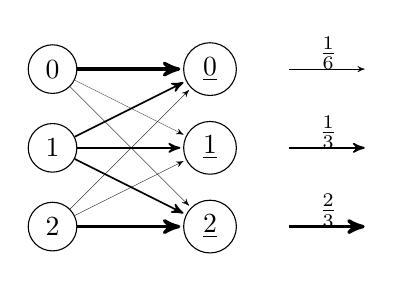
\begin{tikzpicture}[->,>=stealth',shorten >=1pt,auto,node
      distance=2cm,node/.style={circle,draw}]
      \node[node] (i0) at ( -2,  1) { $0$ };
      \node[node] (i1) at ( -2,  0) { $1$ };
      \node[node] (i2) at ( -2, -1) { $2$ };

      \node[node] (o0) at (  0,  1) { $\underline{0}$ };
      \node[node] (o1) at (  0,  0) { $\underline{1}$ };
      \node[node] (o2) at (  0, -1) { $\underline{2}$ };

      \hide{
      \node at (1.5,  1) {
        $
        \begin{array}{l}
          0(1),1(0),2(0)
        \end{array}
        $ };
      \node at (1.5,  0) {
        $
        \begin{array}{l}
          0(0),1(1),2(0)
        \end{array}
        $ };
      \node at (1.5, -1) {
        $
        \begin{array}{l}
          0(0),1(0),2(1)
        \end{array}
        $ };
      }

      \draw[->,very thick] (i0) -- (o0);   % 2/3
      \draw[->,ultra thin]  (i0) -- (o1);   % 1/6
      \draw[->,ultra thin]  (i0) -- (o2);   % 1/6

      \draw[->,semithick] (i1) -- (o0);               % 1/3
      \draw[->,semithick] (i1) -- (o1);               % 1/3
      \draw[->,semithick] (i1) -- (o2);               % 1/3

      \draw[->,ultra thin]  (i2) -- (o0);   % 1/6
      \draw[->,ultra thin]  (i2) -- (o1);   % 1/6
      \draw[->,very thick] (i2) -- (o2);   % 2/3

      \node at (1.5, 1.2) { $\frac{1}{6}$ };
      \draw[->,ultra thin] (1,  1) -- (2,  1);
      \node at (1.5, 0.2) { $\frac{1}{3}$ };
      \draw[->,semithick]  (1,  0) -- (2,  0);
      \node at (1.5,-0.8) { $\frac{2}{3}$ };
      \draw[->,very thick] (1, -1) -- (2, -1);
      
\hide{      
      \path
      (i0) edge node[above] { $\frac{2}{3}$ } (o0)
      (i0) edge node { $\frac{1}{6}$ } (o1)
      (i0) edge node[below] { $\frac{1}{6}$ } (o2)

      (i1) edge node[above] { $\frac{1}{3}$ } (o0)
      (i1) edge node { $\frac{1}{3}$ } (o1)
      (i1) edge node[below] { $\frac{1}{3}$ } (o2)

      (i2) edge node[above] { $\frac{1}{6}$ } (o0)
      (i2) edge node { $\frac{1}{6}$ } (o1)
      (i2) edge node[below] { $\frac{2}{3}$ } (o2)
      ;
    }
      \end{tikzpicture}
    }
  \caption{Truncated $\frac{1}{2}$-Geometric Mechanism}
  \label{figure:geometric-mechanism}
\end{figure}

\noindent
\textit{Example 1.}
To see how differential privacy works, let us consider the truncated
$\frac{1}{2}$-geometric mechanism
(Figure~\ref{figure:geometric-mechanism}). 
In the figure, the states $0$, $1$, and $2$ denote the number of
individuals contracting the disease; the states $\underline{0}$,
$\underline{1}$, $\underline{2}$ denote the outputs of the
mechanism. At the state $\underline{0}$, \textit{zero} is observed
with probability $1$ but \textit{one} and \textit{two} can never be 
observed. Similarly, the states $\underline{1}$ and $\underline{2}$
only observe \textit{one} and \textit{two} respectively. 
In the figure, thin arrows denote transitions with probability
$\frac{1}{6}$; medium arrows denote transitions with probability
$\frac{1}{3}$; thick arrows denote transitions with probability
$\frac{2}{3}$. For instance, the state $0$ can transit to the state
$\underline{0}$ with probability $\frac{2}{3}$ while it can transit to
the state $\underline{1}$ with probability $\frac{1}{6}$.

Let us consider a data set whose two members (including John) contract
the disease. Thus the number of individuals contracting the disease is
$2$. From the state $2$, we see the mechanism answers
\textit{zero}, \textit{one}, and \textit{two} with probabilities
$\frac{1}{6}$, $\frac{1}{6}$, and $\frac{2}{3}$ respectively. 
Suppose we replace John with an individual who does not contract
the disease. The number of individuals contracting the disease for the
new data set is $1$. From the state $1$, we see the mechanism answers
\textit{zero}, \textit{one}, and \textit{two} with the probability
$\frac{1}{3}$.

If an attacker queries the number of individuals contracting the
disease through the truncated $\frac{1}{2}$-geometric mechanism, 
he will get the answer \textit{two} with probability at least
$\frac{1}{3}$ regardless of John's record. The truncated
$\frac{1}{2}$-geometric mechanism is known to be
$\ln(2)$-differentially private. For any two similar data sets, the
mechanism always have similar output distributions. Information
revealed to attackers is therefore limited.

\noindent
\textit{Example 2.}
It is interesting to see when differential privacy may fail. Consider
a data set consisting of two family members and a contagious
disease. An attacker will immedidately infer the number of individuals
contracting the disease can only be $0$ or $2$. If none has contracted
the disease, the attacker observes \textit{zero}, \textit{one}, and
\textit{two} with probabilities $\frac{2}{3}$, $\frac{1}{6}$, and
$\frac{1}{6}$ respectively. If the two members have the disease, the
probabilities are $\frac{1}{6}$, $\frac{1}{6}$, and $\frac{2}{3}$
respectively. Note that it is $4 = \frac{2/3}{1/6}$ times more likely
to observe \textit{zero} when there is none contracting the disease
than there are two. Similarly, it is $4$ times more likely to observe
\textit{two} in the other case. Even though the
$\frac{1}{2}$-geometric mechanism is $\ln(2)$-differentially private,
it may reveal too much information \emph{when the attacker has prior
 knowledge about the data set and disease.}


\noindent
\textit{Example 3.}
Let us analyze the scenario in the previous example with the
Pufferfish privacy framework. Suppose the attacker knows that the data
set contains two family members and the disease is contagious. We
would like to compare the probabilities of observing \textit{zero}
when a member has contracted the disease or not. If a family member
has contracted the disease, the number of individuals contracting
the disease must be $2$ by the prior knowledge. The attacker thus
observes \textit{zero} with probability $\frac{1}{6}$.
If, on the other hand, a family member has not contracted
the disease, the number of individuals contracting the disease must be
$0$ by the prior knowledge. The attacker observes \textit{zero}
with probability $\frac{2}{3}$. The probabilities of observing
\textit{zero} are $\frac{1}{6}$ and $\frac{2}{3}$ when a family
has contracted the disease or not respectively. The
$\frac{1}{2}$-geometric mechanism does not satisfy 
$\ln(2)$-Pufferfish privacy. 

\noindent
\textit{Example 4.}
Prior knowledge does not necessarily lead to privacy leak. Consider a
non-contagious disease. An attacker may know that contracting the
disease is an independent event with probability $p$. Even though the
attacker does not know how many individuals have disease exactly, the
person can still infer that the number of individuals contracting the
disease is $0$, $1$, and $2$ with probabilities $(1-p)^2$, $2p(1-p)$,
and $p^2$ respectively. The prior knowledge can be easily formalized
by an information state in Figure~\ref{figure:geometric-mechanism}.
Consider the information
state where the probabilities at the states $0$, $1$, $2$,
$\underline{0}$, $\underline{1}$, and $\underline{2}$ are $(1-p)^2$,
$2p(1-p)$, $p^2$, $0$, $0$, and $0$ respectively.

Using the Pufferfish framework, we analyze the $\frac{1}{2}$-geometric
mechanism with the prior knowledge as follows. Assume the data set
contains John's record and John has contracted the disease. We would
like to compare probabilities of observations \textit{zero},
\textit{one}, and \textit{two} conditioned on the prior knowledge and
the presence/absence of John's record.

Suppose John's record is not in the data set. With the attacker's
prior knowledge, we see that the mechanism outputs \textit{zero} with
probability $(1-p)^2 \times \frac{2}{3} + 2p(1-p) \times \frac{1}{3} +
p^2 \times \frac{1}{6} = \frac{1}{6} p^2 - \frac{2}{3} p +
\frac{2}{3}$. Similarly, the mechanism outputs \textit{one} and
\textit{two} with probabilities $-\frac{1}{3} p^2 + \frac{1}{3} p +
\frac{1}{6}$ and $\frac{1}{6} p^2 + \frac{1}{3} p + \frac{1}{6}$
respectively.

Now suppose John's record is indeed in the data set. Since John has
the disease, the number of individuals contracting the disease cannot
be $0$. Conditioned on the prior knowledge, we have another
information state whose probabilities at the states $0$, $1$, $2$,
$\underline{0}$, $\underline{1}$, and $\underline{2}$ are $0$,
$\frac{2p(1-p)}{2p(1-p) + p^2} = \frac{2-2p}{2-p}$,
$\frac{p^2}{2p(1-p) + p^2} = \frac{p}{2-p}$, $0$, $0$, and $0$
respectively. From this information state, the mechanism outputs
\textit{zero}, \textit{one}, and \textit{two} with probabilities
$\frac{4-3p}{12-6p}$, $\frac{4-3p}{12-6p}$, and $\frac{2}{6-3p}$
respectively. Table~\ref{table:Pufferfish-geometric-mechanism}
summarizes observation probabilities.

\begin{table}
  \caption{Pufferfish Anlysis of $\frac{1}{2}$-Geometric Mechanism}
  \label{table:Pufferfish-geometric-mechanism}
  \centering
  \[
    \begin{array}{c|ccc}
      & \textit{zero} & \textit{one} & \textit{two} \\
      \hline
      \textmd{without John's record}
      & \frac{p^2 - 4p + 4}{6}
      & \frac{-2p^2 + 2p + 1}{6}
      & \frac{p^2 + 2p + 1}{6}
      \\

      \textmd{with John's record}
      & \frac{4-3p}{12-6p}
      & \frac{4-3p}{12-6p}
      & \frac{2}{6-3p}
    \end{array}
  \]
\end{table}

For observation \textit{zero}, it is not hard to check $\frac{1}{2}
\times \frac{4-3p}{12-6p} \leq \frac{p^2 - 4p + 4}{6} \leq 2 \times
\frac{4-3p}{12-6p}$ for any $0 < p < 1$. Similarly, we have
$\frac{1}{2} \times 
\frac{4-3p}{12-6p} \leq \frac{-2p^2 + 2p + 1}{6} \leq 2 \times
\frac{4-3p}{12-6p}$ and $\frac{1}{2} \times \frac{2}{6-3p} \leq
\frac{p^2 + 2p + 1}{6} \leq 2 \times \frac{2}{6-3p}$  for observations
\textit{one} and \textit{two} respectively. Therefore, the
$\frac{1}{2}$-geometric mechanism satisfies $\ln(2)$-Pufferfish
privacy when contracting the disease is \emph{independent}. 
 
In~\cite{KM:14:PFMPD}, it is shown that differential privacy is
subsumed by Pufferfish privacy (Theorem~6.1). This example is an
instance of the general theorem but formalized in hidden Markov
models. 

\noindent
\textit{Example 5.}
It is worth noting that independency of contracting disease is not
necessary for Pufferfish privacy. Let the probabilities of $0$, $1$,
and $2$ individuals contracting the disease are $p_0$, $p_1$, $p_2$
respectively. Then $p_0 + p_1 + p_2 = 1$. Moreover, the probabilities
of observing \textit{zero}, \textit{one}, and \textit{two} are
$\frac{2}{3} p_0 + \frac{1}{3} p_1 + \frac{1}{6} p_2$,
$\frac{1}{6} p_0 + \frac{1}{3} p_1 + \frac{1}{6} p_2$, and
$\frac{1}{6} p_0 + \frac{1}{3} p_1 + \frac{2}{3} p_2$ respectively.
Assume it is known that an individual in the data set has contracted
the disease. The probabilities of $0$, $1$, and $2$ individuals
contracting the disease become $0$, $\frac{p_1}{p_1 + p_2}$, and
$\frac{p_2}{p_1 + p_2}$ respectively. Consequently, the probabilities
of observing \textit{zero}, \textit{one}, and \emph{two} are
$\frac{\frac{1}{3}p_1 + \frac{1}{6}p_2}{p_1 + p_2}$,
$\frac{\frac{1}{3}p_1 + \frac{1}{6}p_2}{p_1 + p_2}$, and
$\frac{p_1 + 2p_2}{3(p_1 + p_2)}$ respectively. Choose $p_0 =
\frac{1}{2}$, $p_1 = p_2 = \frac{1}{4}$. For the observation
\textit{zero} we have, 
$\frac{1}{8} =
\frac{1}{2} \times \frac{\frac{1}{3}p_1 + \frac{1}{6}p_2}{p_1 + p_2}
\leq
\frac{11}{24} =
\frac{2}{3} p_0 + \frac{1}{3} p_1 + \frac{1}{6} p_2
\leq
{2} \times \frac{\frac{1}{3}p_1 + \frac{1}{6}p_2}{p_1 + p_2}
= \frac{1}{2}$.
Similarly, we have
$
\frac{1}{8} =
\frac{1}{2} \times \frac{\frac{1}{3}p_1 + \frac{1}{6}p_2}{p_1 + p_2}
\leq
\frac{5}{24} =
\frac{1}{6} p_0 + \frac{1}{3} p_1 + \frac{1}{6} p_2
\leq
2 \times \frac{\frac{1}{3}p_1 + \frac{1}{6}p_2}{p_1 + p_2}
= \frac{1}{2}$ for the observation \textit{one}. And
$
\frac{1}{4}
=
\frac{1}{2} \times \frac{p_1 + 2p_2}{3(p_1 + p_2)}
\leq
\frac{1}{3}
=
\frac{1}{6} p_0 + \frac{1}{3} p_1 + \frac{2}{3} p_2
\leq 
2 \times \frac{p_1 + 2p_2}{3(p_1 + p_2)}
= 1$ for the observation \textit{two}. In other words, the
$\frac{1}{2}$-geometric mechanism satisfies Pufferfish privacy for
attackers with the prior distribution $(\frac{1}{2}, \frac{1}{4},
\frac{1}{4})$ on the number of individuals contracting the disease.
Suppose the distribution $(\frac{1}{2}, \frac{1}{4},
\frac{1}{4})$ is binomial. There is $0 \leq p \leq 1$ such that
$(1-p)^2 = \frac{1}{2}$, $2p(1-p) = \frac{1}{4}$, and $p^2 =
\frac{1}{4}$. From $p^2 = \frac{1}{4}$ and $0 \leq p$, we have $p =
\frac{1}{2}$. But we would have $(1-p)^2 = \frac{1}{4} \neq
\frac{1}{2}$. Hence $(\frac{1}{2}, \frac{1}{4}, \frac{1}{4})$ is not
binomial. Even though the prior distribution is not derived by
independent contraction of the disease, $\frac{1}{2}$-geometric
mechanism does not reveal too much information. Independency of
contraction is not necessary for Pufferfish privacy on the geometric
mechanism. 



\section{Complexity of Pufferfish Privacy in HMMs}
\label{section:complexity}

Actually, we formulate the above Pufferfish privacy cases into Hidden Markov Models.
For instance, in \textit{Example 3}, the state space consists of ($0, 1, 2, \underline{0}, \underline{1}, \underline{2}$).
The states $\underline{0}$, $\underline{1}$ and $\underline{2}$ emit, with certainty,
observation $\textit{zero}$, $\textit{one}$ and $\textit{two}$ respectively.
Even though the attacker has the prior knowledge that the disease is contagious,
we want to make sure that he won't infer whether any member in the data set
has contracted the disease or not. Thus the initial distribution pair the attacker gets would be
($1,0,0,0,0,0$) and ($0,0,1,0,0,0$). And since the probabilities of observing
$\textit{zero}$ are $\frac{2}{3}$ and $\frac{1}{6}$, this violates $\ln(2)$-Pufferfish privacy.

To formalize, given a set of secrets $\bbfS$,
a set of discriminative secret pairs $\bbfS_{\textmd{pairs}}$, a set of data evolution
scenarios $\bbfD$ , and $\epsilon > 0$, we model the mechanism  $\calM$ into a Hidden Markov Chain
and compute whether it's $\epsilon$-Pufferfish ($\bbfS$, $\bbfS_{\textmd{pairs}}$
$\bbfD$) private. We use states and transitions to model the mechanism $\calM$,
set certain target initial distribution pairs according to prior knowledge $\bbfD$ and discriminative secrets $\bbfS_{\textmd{pairs}}$,
set target outputs as observations, and then check whether the probabilities under the same observation sequence
are mathematical similar(i.e, $\epsilon$-Pufferfish private), for every distribution pair and every observation sequence.
Therefore, our task turns into finding the observation sequence that makes the observing probabilities differ the most;
that is, in Pufferfish framework, for every observation sequence $O=o_1o_2\ldots$, secret pair $(s_i, s_j) \in
\bbfS_{\textmd{pairs}}$ and $\theta \in \bbfD$
  \begin{equation}\label{max1}
     \max_{O,(s_i, s_j) \in
    \bbfS_{\textmd{pairs}},\theta \in \bbfD}
    { \Pr (\calM (\oD) = O| s_i, \theta) - e^\epsilon \Pr (\calM (\oD) = O| s_j, \theta) }
  \end{equation}

  \begin{equation}\label{max2}
     \max_{O,(s_i, s_j) \in
    \bbfS_{\textmd{pairs}},\theta \in \bbfD}
     { \Pr (\calM (\oD) = O| s_j, \theta) - e^\epsilon \Pr (\calM (\oD) = O| s_i, \theta) }
  \end{equation}
are less than or equal to 0.

However, as we will show below, the problem is NP-hard.

\begin{theorem}
  The Pufferfish privacy problem in Hidden Markov Model is NP-hard.
\end{theorem}

\begin{proof}
  In order to satisfy Pufferfish privacy in hidden Markov model, we have to decide whether
  the maximum value of (\ref{max1}) (\ref{max2}) is less than or equal to $0$.
  Let's just simplify the problem by only having one initial distribution pair to compare
  so that we only need to find the observation sequence.
  We will show this simplified version to find this maximum value is still NP-hard.
  To show NP-hardness, we reduce SAT to this problem. Assume we have a formula $F(x_1,\ldots,x_n)$ in conjuncted normal form,
  with $n(n>=3)$ variables and $m$ clauses, $C_1,\ldots,C_m$. We shall construct a hidden Markov model $H = (K, \Obs, o)$
  such that(\ref{max1})and (\ref{max2}) will take the maximum value $0$
  if and only if the formula $F(x_1,\ldots,x_n)$ is satisfiable.

  \textit{Construction.} The construction is similar in \cite{PCT:87:CMDP}. We first describe the Markov Chain $K =
  (S, p)$. $S$ contains a state group $A$ with six states $A_{ij},A'_{ij},T_{A ij},T'_{Aij},F_{Aij},F'_{Aij}$ and
  a state group $B$ with six states $B_{ij},B'_{ij},T_{Bij},T'_{Bij},F_{Bij},F'_{Bij}$
  for each clause $C_i$ and variable $x_j$. Besides, there are $4m$ states $A_{i,n+1},A'_{i,n+1},B_{i,n+1},B'_{i,n+1}$.
  The transition distribution $p$ is as followed. For group $A$, there are two transitions with same probability $\frac{1}{2}$ leading from
  state $A_{ij}$ to $T_{Aij}$ and $F_{Aij}$ respectively; similarly there are two transitions leading with probability $\frac{1}{2}$
  from $A'_{ij}$ to $T'_{Aij}$ and $F'_{Aij}$. There's only one transition leading with certainty from $T_{Aij},F_{Aij},T'_{Aij},F'_{Aij}$,
  to $A_{i,j+1},A_{i,j+1},A'_{i,j+1},A'_{i,j+1}$ respectively with two exceptions: If $x_j$ appears positively in $C_i$,
  the transition from $T'_{Aij}$ is to $A_{i,j+1}$ instead of $A'_{i,j+1}$; and if $x_j$ appears negatively, the transition from
  $F'_{Aij}$ is to $A_{i,j+1}$. For the state group $B$, all the transitions imitate that in group $A$ only with different state names.
  For instance, there are two transitions leading with same probability $\frac{1}{2}$ from state $B_{ij}$ to $T_{Bij}$ and $F_{Bij}$ and so on.

  Next we describe the observations $\Obs$ and the observation distribution. In state
  $A_{ij},A'_{ij},B_{ij},B'_{ij}$ with $1\leq j \leq n$, one can observe $X_j \in \Obs$ with certainty.
  In state $T_{Aij},T'_{Aij},T_{Bij},T'_{Bij}$ with $1\leq j \leq n$, one can only observe $T_j \in \Obs$;
  similarly, the sole observation $F_j \in \Obs$ can be observed in state $F_{Aij},F'_{Aij},F_{Bij},F'_{Bij}$ with $1\leq j \leq n$.
  In state $A_{i,n+1}$, we have probability $\frac{4}{5}$ to observe $\top \in \Obs$ and $\frac{1}{5}$  to observe $\bot \in \Obs$;
  while in state $B_{i,n+1}$, we have probability $\frac{1}{5}$ to observe $\top$ and $\frac{4}{5}$  to observe $\bot \in \Obs$.
  In state $A'_{i,n+1}$ and $B'_{i,n+1}$, there are equal probabilities of $\frac{1}{2}$ observing $\top$ and $\bot$.

  Then we describe the Pufferfish privacy scenario in this Hidden Markov Model. Assume that according to
  prior knowledge $\bbfD$ and discriminative secrets $\bbfS_{\textmd{pairs}}$, we only have
  two initial distributions $\oD_1$ and $\oD_2$ to compare. $\oD_1$ induces a uniform distribution,
  to start from each member in the state set $\{A'_{i1}\}$ with $1 \leq i \leq m$, whose probability is $\frac{1}{m}$.
  Similarly, in $\oD_2$, the probability starting from each member in the state set $\{B'_{i1}\}$ is also $\frac{1}{m}$ with $1 \leq i \leq m$.

  \textit{Reduction.} The intuition is that starting from state $A'_{i1}$ or $B'_{i1}$,
  the clause $C_i$ is chosen and then the assignment of each variable will be considered one by one
  in this clause. Once the assignment of a variable $x_j$ makes $C_i$ satisfied, immediately
  state $A_{i,j+1}$ or $B_{i,j+1}$ is reached. So at last if state $A'_{i,n+1}$ or $B'_{i,n+1}$
  is reached, it means that the clause $C_i$ is not satisfied under this assignment. Now, we take $\epsilon = \ln 4$
  and claim that  $\Pr (\calM (\oD_1) = O) - 4 \times \Pr (\calM (\oD_2) = O)$ takes the maximum value $0$
  if and only if $O$ is the observation sequence $X_1A_1X_2\ldots A_n \top$ such that
  formula $F(x_1,\ldots,x_n)$ is satisfied under assignment $A_i \in \{T_i,F_i\}$ for each variable $x_i$
  (Similar analysis applies for $\Pr (\calM (\oD_2) = O) - 4 \times \Pr (\calM (\oD_1) = O)$ except that it takes the
   maximum value $0$ with $\bot$ as the last observation).

  We argue that $0$ is the maximum value.
  It's easy to see that if we take an arbitrary observation sequence $O = X_1A_1X_2\ldots $,
  as long as $\top$ or $\bot$ hasn't been observed, $\Pr (\calM (\oD_1) = O) -  4 \times \Pr (\calM (\oD_2) = O) < 0$.
  That's because the state group $B$ just imitate the state group $A$ before reaching the state
  $B_{i,n+1}$ and $B'_{i,n+1}$. Thus the maximum value must be less than 0 or be obtained after we observe $\top$
  or $\bot$.

  Then we consider $O=X_1A_1X_2\ldots A_n \top$. Note that if $C_i$ is satisfied under observation $O$, we start from $A'_{i1}$ and $B'_{i1}$ both with
  probability $\frac{1}{m}$, finally reaching $A_{i,n+1}$ and $B_{i,n+1}$ with probabilities $2^{-n} \times \frac{1}{m} \times \frac{4}{5}$
  and $2^{-n} \times \frac{1}{m} \times \frac{1}{5}$ respectively;
  if $C_i$ is not satisfied, we finally reach $A'_{i,n+1}$ and $B'_{i,n+1}$  with equal probabilities of $2^{-n}\times \frac{1}{m} \times \frac{1}{2}$ .
  Thus a satisfied clause will contribute $2^{-n} \times \frac{1}{m} \times \frac{4}{5} - 4 \times 2^{-n} \times \frac{1}{m} \times \frac{1}{5} = 0$ to
  the result; While if some clause is not satisfied, $\Pr (\calM (\oD_1) = O)- 4\times \Pr (\calM (\oD_2) = O)$ is strictly less than $0$.
  Therefore, if we choose a observation sequence ended with $\top$ such that all the
  clauses are satisfied, $\Pr (\calM (\oD_1) = O)- 4\times \Pr (\calM (\oD_2) = O)$ will take the maximum value 0.
  If we consider $O=X_1A_1X_2\ldots A_n \bot$, similar analysis concludes that $\Pr (\calM (\oD_1) = O) - 4 \times \Pr (\calM (\oD_2) = O)$
  will be strictly less than $0$.
  This indicates that the maximum value of $\Pr (\calM (\oD_1) = O) - 4 \times \Pr (\calM (\oD_2) = O)$ is $0$.

  Finally from the process above,
  $\Pr (\calM (\oD_1) = O) - 4 \times \Pr (\calM (\oD_2) = O)$ takes the maximum value $0$
  if and only if $O$ is the observation sequence $X_1A_1X_2\ldots A_n \top$ such that
  formula $F(x_1,\ldots,x_n)$ is satisfied under assignment $A_i \in \{T_i,F_i\}$ for each variable $x_i$,
  which means that $F(x_1,\ldots,x_n)$ is satisfiable.
  We can also infer that if $\epsilon$ is slightly smaller than $\ln 4$, the maximum value of
  $\Pr (\calM (\oD_1) = O) - e ^\epsilon \times \Pr (\calM (\oD_2) = O)$ will be more than $0$,
  therefore $\epsilon-$Pufferfish privacy is not satisfied.
  This indicates that the general problem for $\epsilon-$Pufferfish privacy is NP-hard.

 \iffalse
  The "if" direction can be immediately proved from the process of finding the maximum.
  For the "only if" direction, with proof by contradiction, assume that $\Pr (\calM (\oD_1) = O) - \Pr (\calM (\oD_2) = O)$ takes
  value $2^{-n}$ but $O$ doesn't satisfy above condition. With the analysis before, the observation must be in the form
  of $O=X_1A_1X_2\ldots A_n \top$, where the assignment implied by $O$ doesn't satisfy $F(x_1,\ldots,x_n)$.
  So some clause $C_i$ is not satisfied and starting from $A'_{ij}$ the probability of
  observe $O$ is $2^{-n-1}\times \frac{1}{m}$. Therefore the sum of all the clauses observing
  $O$ is smaller than $2^{-n}$ since a clause which is satisfied only has a distribution
  of  $2^{-n}\times \frac{1}{m}$ observing $O$. That's a contradiction.
 \fi
\end{proof} 

\section{Checking Pufferfish Privacy}
\label{section:checking-pufferfish}

\begin{algorithm}
  \begin{algorithmic}[1]
    \Require{$H = ((S, p), \Obs, o)$ : an HMM; 
      $\pi, \tau$ : state distributions on $S$; $c$ : a
      non-negative real number; $k$ : a positive integer}
    \Ensure{An SMT query $q$ such that $q$ is unsatisfiable iff
      $\Pr (\overline{\omega} | \pi, H) \leq c \cdot
       \Pr (\overline{\omega} | \tau, H)$ for every observation
       sequences $\overline{\omega}$ of length $k$}
     \Function{PufferfishCheck}{$H$, $\pi_0$, $\pi_1$, $c$, $k$}
       \For{$s \in S$}
         \State{$\alpha_0(s) \leftarrow
           \textmd{\textsc{Product}} (\pi(s),
           \textmd{\textsc{Select}}(\mathsf{w_0}, \Omega, o(s, \bullet)))$}
         \State{$\beta_0(s) \leftarrow
           \textmd{\textsc{Product}} (\tau(s),
           \textmd{\textsc{Select}}(\mathsf{w_0}, \Omega, o(s, \bullet)))$}
       \EndFor
       \For{$t \leftarrow 1$ \textbf{to} $k - 1$}
         \For{$s' \in S$}
           \State{$\alpha_t(s') \leftarrow
             \textmd{\textsc{Product}} (
             \textmd{\textsc{Dot}} (\alpha_{t-1}, p (\bullet, s')),
             \textmd{\textsc{Select}} (\mathsf{w_t}, \Omega, o(s', \bullet)))
             $}
           \State{$\beta_t(s') \leftarrow
             \textmd{\textsc{Product}} (
             \textmd{\textsc{Dot}} (\beta_{t-1}, p (\bullet, s')),
             \textmd{\textsc{Select}} (\mathsf{w_t}, \Omega, o(s', \bullet)))
             $}
         \EndFor
       \EndFor
       \State{\Return{
           $\bigwedge_{t=0}^{k-1} \mathsf{w_t} \in \Obs \wedge
           \textmd{\textsc{Gt}} (
           \textmd{\textsc{Sum}} (\alpha_{k-1}),
           \textmd{\textsc{Product}} (c,
           \textmd{\textsc{Sum}} (\beta_{k-1}))
           )$
       }}
     \EndFunction
 \end{algorithmic}
 \caption{Pufferfish Check}
 \label{algorithm:pufferfish-check}
\end{algorithm}

Our next goal is to develop an algorithm to check
$\epsilon$-Pufferfish privacy on any given HMM. Since the problem is
NP-hard, we will employ Satisfiability Modulo Theories (SMT) solvers
in our algorithm. For all observation sequences of length $k$, we will 
construct an SMT query to find a sequence violating
$\epsilon$-Pufferfish privacy. If no such sequence can be found, the
given HMM satisfies $\epsilon$-Pufferfish privacy for observation
sequences of length $k$.

Let $H = ((S, p), \Obs, o)$ be an HMM, $\pi, \tau$ two initial state
distributions on $S$, $c \geq 0$ a real number, and $k$ a positive
integer. For a fixed observation sequence $\overline{\obs}$,
computing the probability $\Pr (\overline{\obs} | \pi, 
H)$ of observing $\overline{\obs}$ from $\pi$ can be done in
polynomial time~\cite{R:89:ATHMM}. It is straightforward to check if
$\Pr (\overline{\obs} | \pi, H) > c \cdot \Pr (\overline{\obs} |
\tau, H)$ for any fixed observation sequence $\overline{\obs}$. One
simply computes the respective probabilities and then checks the
inequality. 

Our algorithm exploits the efficient algorithm for computing the
probability of observation sequences. Rather than a fixed observation 
sequence, we declare $k$ SMT variables $\mathsf{w_0}, \mathsf{w_1},
\ldots, \mathsf{w_{k-1}}$ for observations at each step. The
observation at each step is determined by one of the $k$ variables. To
this end, we define the SMT expression
$\textmd{\textsc{Select}} (\mathsf{w}, \{ \obs_1, \obs_2, \ldots,
\obs_m\}, o (s, \bullet))$  equal to $o (s, \obs)$ when the SMT
variable $\mathsf{w}$ is $\obs$. It is easy to formulate by
the SMT $\mathsf{ite}$ (if-then-else) expression:
\begin{align*}
  \mathsf{ite} (\mathsf{w} = \obs_1, o (s, \obs_1),
  \mathsf{ite} (\mathsf{w} = \obs_2, o (s, \obs_2),
  \ldots
  ,\mathsf{ite} (\mathsf{w} = \obs_m, o (s, \obs_m), \mathsf{w})
  \ldots))
\end{align*}

Using $\textmd{\textsc{Select}} (\mathsf{w}, \{ \obs_1, \obs_2,
\ldots, \obs_m\}, o (s, \bullet))$, it is easy to construct an SMT
expression to compute $\Pr (\overline{\mathsf{w}} | \pi, H)$ where
$\overline{\mathsf{w}}$ is a sequence of SMT variables ranging over
the observations $\Obs$ (Algorithm~\ref{algorithm:pufferfish-check}).
Recall the equations (\ref{hmm:basis}) and (\ref{hmm:inductive}). We
simply replace the expression $o (s, \obs)$ with
$\textmd{\textsc{Select}} (\mathsf{w}, \{ \obs_1, \obs_2, \ldots,
\obs_m\}, o (s, \bullet))$ to leave the observation determined by the
SMT variable $\mathsf{w}$. In the algorithm, we also use auxiliary
functions. 
$\textmd{\textsc{Product}}(\mathit{smtExp}_0, \mathit{smtExp}_1,
\ldots, \mathit{smtExp}_m)$
returns the SMT expression denoting the product of
$\mathit{smtExp}_0$, $\mathit{smtExp}_1, \ldots,$
$\mathit{smtExp}_m$. Similarly, 
$\textmd{\textsc{Sum}}(\mathit{smtExp}_0,$ $\mathit{smtExp}_1, \ldots,$
$\mathit{smtExp}_m)$ returns the SMT expression for the sum
of $\mathit{smtExp}_0$, $\mathit{smtExp}_1, \ldots,$
$\mathit{smtExp}_m$. $\textmd{\textsc{Gt}} (\mathit{smtExp}_0,
\mathit{smtExp}_1)$ returns the SMT expression for
$\mathit{smtExp}_0$ greater than $\mathit{smtExp}_1$.
Finally, 
$\textmd{\textsc{Dot}} ([\mathsf{a_0}, \mathsf{a_1}, \ldots,$
$\mathsf{a_n}], [\mathsf{b_0}, \mathsf{b_1}, \ldots, \mathsf{b_n}])$
returns the SMT expression for the inner product of the two lists of
SMT expressions, namely,
\[
  \textmd{\textsc{Sum}} (
  \textmd{\textsc{Product}}(\mathsf{a_0}, \mathsf{b_0}),
  \textmd{\textsc{Product}}(\mathsf{a_1}, \mathsf{b_1}),
  \ldots,
  \textmd{\textsc{Product}}(\mathsf{a_n}, \mathsf{b_n})
  ).
\]

Algorithm~\ref{algorithm:pufferfish-check} is summarized in the
following theorem. 

\begin{theorem}
  Let $H = ((S, p), \Obs, o)$ be an HMM, $\pi, \tau$ state
  distributions on $S$, $c > 0$ a real number, and $k > 0$ an
  integer. Algorithm~\ref{algorithm:pufferfish-check} returns an SMT
  query such that the query is unsatisfiable iff
  $\Pr (\overline{\omega} | \pi, H) \leq c \cdot
  \Pr (\overline{\omega} | \tau, H)$ for every observation
  sequences $\overline{\omega}$ of length $k$.
\end{theorem}


We have implemented our algorithm using \zpython. All examples in
Section~\ref{section:hmm} are checked with our implementation. In
\textit{Example~4}, contracting the disease is independent with
probability $p > 0$. Even though the query contains non-linear
constraints over real numbers, \zpython still proves that the
$\frac{1}{2}$-geometric mechanism satisfies $\ln(2)$-Pufferfish
privacy for any probability $0 < p < 1$. In \textit{Example~5}, it is
assumed that the probability of $m$ individuals contracting the
disease is $p_m > 0$ for $m = 0, 1, 2$. The probabilities $(p_0, p_1,
p_2) = (\frac{1}{2}, \frac{1}{4}, \frac{1}{4})$ are in fact found by
\zpython. The SMT solver is able to find a non-binomial initial state
distribution to satisfy $\ln(2)$-Pufferfish privacy. 

\section{Case Study: Noisy Max}
\label{section:noisy-max}

% It is important to return indices. Otherwise, this is not DP.

\begin{algorithm}
  \begin{algorithmic}[1]
    \Require{$0 \leq v_1, v_2, \ldots, v_n \leq 2$}
    \Ensure{The index $r$ with the maximal $v_r$ among $v_1, v_2, \ldots, v_n$}
    \Function{NoisyMax}{$v_1, v_2, \ldots, v_n$}
      \For{each $v_i$}
        \Match{$v_i$}
        \Comment{apply $\frac{1}{2}$-geometric mechanism to $v_i$}
          \lCase{$0$}
                {$\tilde{v}_i \leftarrow 0, 1, 2$ with probability
                 $\frac{2}{3}, \frac{1}{6}, \frac{1}{6}$}
          \lCase{$1$}
                {$\tilde{v}_i \leftarrow 0, 1, 2$ with probability
                 $\frac{1}{3}, \frac{1}{3}, \frac{1}{3}$}
          \lCase{$2$}
                {$\tilde{v}_i \leftarrow 0, 1, 2$ with probability
                 $\frac{1}{6}, \frac{1}{6}, \frac{2}{3}$}
        \EndMatch
      \EndFor
      \State{find $1 \leq r \leq n$ such that
        $\tilde{v}_r \geq \tilde{v}_j$ for every $1 \leq j \leq n$}
      \State{\Return {$r$} }
    \EndFunction
  \end{algorithmic}
  \caption{Noisy Max}
  \label{algorithm:noisy-max}
\end{algorithm}

\begin{figure}
  \centering
    \resizebox{.95\columnwidth}{!}{
    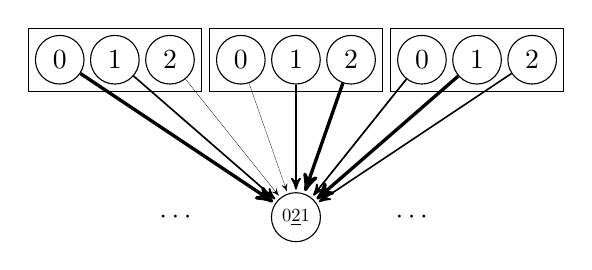
\begin{tikzpicture}[->,>=stealth',shorten >=1pt,auto,node
      distance=2cm,node/.style={circle,draw}]
      \node[node] (v1_0) at (-3.0, 1) { $0$ };
      \node[node] (v1_1) at (-2.3, 1) { $1$ };
      \node[node] (v1_2) at (-1.6, 1) { $2$ };
      \draw (-3.4, 1.4) rectangle (-1.2, .6);

      \node[node] (v2_0) at (-0.7, 1) { $0$ };
      \node[node] (v2_1) at (   0, 1) { $1$ };
      \node[node] (v2_2) at ( 0.7, 1) { $2$ };
      \draw (-1.1, 1.4) rectangle ( 1.1, .6);

      \node[node] (v3_0) at ( 1.6, 1) { $0$ };
      \node[node] (v3_1) at ( 2.3, 1) { $1$ };
      \node[node] (v3_2) at ( 3.0, 1) { $2$ };
      \draw ( 1.2, 1.4) rectangle ( 3.4, .6);

\hide{
      \node[node, scale=0.67] (000) at (-3.0, -1) { $\underline{0}00$ };

      \node at (-1.5, -1) { $\cdots$ };

      \node[node, scale=0.67] (011) at (   0, -1) { $0\underline{1}1$ };

      \node at ( 1, -1) { $\cdots$ };

      \node[node, scale=0.67] (102) at ( 2.0, -1) { $10\underline{2}$ };

      \node at (2.8, -1) { $\cdots$ };
    }

      \node at (-1.5, -1) { $\cdots$ };
      \node[node, scale=0.67] (021) at (0, -1) { $0\underline{2}1$ };
      \node at ( 1.5, -1) { $\cdots$ };
    
      \path
      (v1_0) edge [very thick] (021)
      (v1_1) edge [semithick]  (021)
      (v1_2) edge [ultra thin] (021)

      (v2_0) edge [ultra thin] (021)
      (v2_1) edge [semithick]  (021)
      (v2_2) edge [very thick] (021)

      (v3_0) edge [semithick]  (021)
      (v3_1) edge [very thick] (021)
      (v3_2) edge [semithick]  (021)
      
      ;
      \end{tikzpicture}
    }
  \caption{Hidden Markov Model for Noisy Max}
  \label{figure:hmm-noisy-max}
\end{figure}





\section{Conclusion}
\label{section:conclusion}

We have developed a verification framework for 
Pufferfish privacy, which subsumes
the gradually eye-catching topic in security called differential privacy.
We use hidden Markov models to model the Pufferfish privacy mechanisms and
prove that the verification problem for it in HMMs is NP-hard.
Though, with the help of SMT solvers,
we propose an automatic verification algorithm
to check whether Pufferfish privacy is preserved.
By investigating into several privacy scenarios, including the
classical Noisy Max algorithm in differential privacy and its variant version, 
private mechanisms are analyzed and our algorithm
functions efficiently as verifying Pufferfish privacy.
In the future, it's interesting to model more sophisticated
private mechanisms such as reactive systems. In that case,
HMMs may not be sufficient since
different queries may be asked.
We have the interest in using partially observable
Markov decision process as the model and investigate into
the corresponding verification problem.

\bibliographystyle{splncs03}
\bibliography{refs}

\end{document}
